% =======================================================================================================
% Artigo: inferência embarcada da MLP de EA no MOMEA (Artix-7), verificada inteiramente por simulação.
% Figuras: ../embarcado/figuras_sim.py (pasta figuras/). Números: figuras/../resumo_figuras.json,
% ../embarcado/README.md, relatórios do Vitis HLS e ../embarcado/microblaze/sim/resultados/ciclos_mb.csv.
\documentclass[12pt]{article}
\usepackage[utf8]{inputenc}
\usepackage[T1]{fontenc}
\usepackage[brazilian]{babel}
\usepackage{amsmath, amssymb, amsfonts}
\usepackage{geometry}
\geometry{a4paper, margin=2.5cm}
\usepackage{graphicx}
\graphicspath{{figuras/}}
\usepackage[colorlinks=true, citecolor=blue, linkcolor=blue, urlcolor=blue]{hyperref}
\usepackage{xcolor}
\usepackage{array}
\usepackage{booktabs}
\usepackage{caption}
\usepackage{tikz}
\usetikzlibrary{arrows.meta, positioning, fit, calc}
\captionsetup{font=small, labelfont=bf}
\setlength{\parindent}{1.25cm}
\setlength{\emergencystretch}{3em}
\newcolumntype{L}[1]{>{\raggedright\arraybackslash}p{#1}}
\newcommand{\completar}[1]{\textcolor{red}{[#1]}}

% ---- números medidos na simulação RTL da MicroBlaze (preenchidos de ciclos_mb.csv) ----
% Gerado por embarcado/figuras_sim.py a partir de ciclos_mb.csv e dos ELFs. NÃO EDITAR.
\newcommand{\mbMlpIntSoftUs}{2\,053}
\newcommand{\mbMlpIntFpuUs}{1\,463}
\newcommand{\mbHitSoft}{38\,287}
\newcommand{\mbHitFpu}{4\,232}
\newcommand{\mbCargaEnsaioMax}{1}
\newcommand{\mbMlpFloatSoft}{3\,353\,499}
\newcommand{\mbMlpFloatFpu}{212\,130}
\newcommand{\mbQuantSoft}{66\,296}
\newcommand{\mbQuantFpu}{7\,232}
\newcommand{\mbMlpIntSoft}{139\,042}
\newcommand{\mbMlpIntFpu}{139\,042}
\newcommand{\mbHitHistSoft}{45\,323}
\newcommand{\mbHitHistFpu}{5\,122}
\newcommand{\mbFecharSoft}{749\,938}
\newcommand{\mbFecharFpu}{117\,676}
\newcommand{\mbFecharHistSoft}{214\,316}
\newcommand{\mbFecharHistFpu}{91\,974}
\newcommand{\mbParagrafoMlp}{Sem FPU, a inferência em float32 custou 3\,353\,499 ciclos (33{,}5\,ms), 16 vezes a inferência int8, porque cada operação de ponto flutuante é emulada em software. Com FPU, o float32 caiu para 212\,130 ciclos, 1{,}5 vezes o int8. O núcleo int8 não usa ponto flutuante e custou exatamente o mesmo nas duas configurações (139\,042 ciclos, ou 15{,}5 ciclos por multiplicação-acumulação dos 8\,960 pesos); a diferença entre elas está na quantização da entrada, com algumas dezenas de operações de ponto flutuante, que custou 66\,296 ciclos sem FPU e 7\,232 com FPU.}
\newcommand{\mbParagrafoCarga}{O custo por \textit{hit} é dominado pelos logaritmos, emulados em software sem FPU: 38\,287 ciclos sem FPU e 4\,232 com FPU, no modo exato. O histograma custa um pouco mais por \textit{hit} (45\,323 e 5\,122 ciclos), porque calcula o índice da classe, mas fecha a janela mais depressa (214\,316 contra 749\,938 ciclos sem FPU), porque não ordena: sem FPU, cada comparação da ordenação é uma chamada à biblioteca de ponto flutuante. Na taxa dos ensaios, cerca de 16 \textit{hits}/s nos dois canais, a cadeia completa ocupa 0{,}80\,\% da CPU sem FPU e 0{,}12\,\% com FPU. A 333 \textit{hits}/s por canal (666 no total), a ocupação chega a 25{,}7\,\% sem FPU e 2{,}9\,\% com FPU; nesse regime, a FPU passa a ser recomendável, ou o cálculo dos logaritmos por tabela.}
\newcommand{\mbTextoMin}{36{,}2}
\newcommand{\mbTextoMax}{42{,}4}
\newcommand{\mbTextoExatoSoft}{42{,}0}
\newcommand{\mbTextoExatoFpu}{36{,}2}
\newcommand{\mbTextoHistSoft}{42{,}4}
\newcommand{\mbTextoHistFpu}{36{,}7}
\newcommand{\mbParagrafoRota}{Na MicroBlaze sem FPU, a inferência int8 leva 2\,053\,\(\mu\)s, 0{,}041\,\% de uma janela, e mesmo o float32 emulado (33{,}5\,ms) seria aceitável; a rota em software não exige nenhum recurso adicional de lógica.}
\newcommand{\mbFatorHls}{18}


% =======================================================================================================
\title{\textbf{Inferência embarcada de redes MLP para emissão acústica em FPGA Artix-7: implementação em MicroBlaze e em lógica dedicada, verificada por simulação}}
\date{\today}
\author{Autores \\ Instituições \\ \texttt{email oficial}}
% =======================================================================================================
\begin{document}
\maketitle

\begin{abstract}
O sistema MOMEA extrai \textit{hits} de emissão acústica (EA) na lógica programável de um FPGA Artix-7 e os envia a um computador, onde redes MLP estimam a frequência de rotação e a configuração das válvulas de uma bomba a partir de 36 descritores calculados em janelas de 5\,s. Este artigo leva essa cadeia para dentro do FPGA e, sem acesso às placas, verifica a implementação inteiramente por simulação. O cálculo dos descritores foi portado para C, em dois modos (percentis exatos ou por histograma de memória constante), e as duas redes (36-64-32-1 e 36-64-32-7, cerca de 4,6 mil parâmetros cada) foram quantizadas para int8 com requantização inteira. Um único código-fonte do núcleo int8 compila para o processador MicroBlaze e para o Vitis HLS. A verificação foi organizada em seis níveis, do modelo de referência em Python à simulação RTL do processador executando o binário final. Sobre os 281\,595 \textit{hits} gravados das 56 corridas (3\,540 janelas), o C reproduziu bit a bit a aritmética int8 emulada em Python, e a cadeia completa com percentis exatos devolveu a mesma classe e o mesmo nível de frequência que o Python em 100\,\% das janelas. A quantização int8 alterou a classe em 1,8\,\% das janelas e a frequência em 0,81\,Hz em média em relação ao modelo em ponto flutuante. O núcleo em HLS passou na cossimulação C/RTL, com latência de 11\,391 ciclos (114\,\(\mu\)s a 100\,MHz), e, após posicionamento e roteamento, ocupou 656 LUTs, 682 \textit{flip-flops}, 14 DSPs e 3,5 blocos de BRAM, com período mínimo de 6,84\,ns. Na simulação RTL da MicroBlaze, a inferência int8 das duas redes levou \mbMlpIntSoftUs\,\(\mu\)s sem FPU e \mbMlpIntFpuUs\,\(\mu\)s com FPU, e cada \textit{hit} custou \mbHitSoft{} e \mbHitFpu{} ciclos, respectivamente. Na taxa dos ensaios, a cadeia ocupa menos de \mbCargaEnsaioMax\,\% da CPU. A verificação demonstra a fidelidade e a viabilidade da implementação; ela não substitui o ensaio em placa nem melhora a capacidade de generalização do modelo, que continua limitada pelos dados de treino.
\end{abstract}

% =======================================================================================================
\section{Introdução}
\label{sec:introducao}

O monitoramento contínuo de máquinas hidráulicas por emissão acústica (EA) depende de reduzir na borda o volume de dados. O MOMEA faz isso na lógica programável: detecta os \textit{hits} e transmite, por UDP, um registro de 32 bytes por \textit{hit}, com amplitude de pico, contagens, tempo de subida, duração e energia \cite{unnthorsson2013,vallen2022}. Em um estudo complementar \cite{mlpbomba2026}, redes MLP treinadas sobre descritores desses registros, agregados em janelas de 5\,s, estimaram a frequência de rotação de uma bomba com erro de 4 a 6\,Hz em condições não vistas e reconheceram a configuração das válvulas quando a corrida aparecia no treino.

Nesse arranjo, a classificação ainda acontece no computador. Levá-la para o FPGA fecharia o ciclo na borda: o sistema enviaria, a cada janela, uma estimativa do estado da máquina, além ou no lugar dos registros. O XC7A35T do MOMEA já abriga um processador MicroBlaze, que trata os registros e a pilha de rede, e tem recursos livres de lógica, DSP e BRAM. Há, portanto, duas rotas: executar a inferência em software, na MicroBlaze, ou em um acelerador dedicado gerado por síntese de alto nível (HLS) \cite{amd_ug1399,duarte2018}.

Este trabalho foi feito sem acesso às placas. Por isso, toda a verificação usa simulação, o que exige critérios explícitos de aceitação em cada nível. O objetivo é responder a três perguntas: (i) a implementação embarcada reproduz o modelo de referência e com que diferença numérica; (ii) quanto custa, em tempo e em recursos, em cada rota; e (iii) o que a simulação garante e o que só o ensaio em placa poderá confirmar.

As contribuições são:
\begin{itemize}
	\item a porta em C do cálculo dos 36 descritores por janela, com conversão do registro bruto para unidades físicas e dois modos de percentis, exato e por histograma (Seção~\ref{sec:implementacao});
	\item a quantização int8 das duas MLPs, com requantização inteira emulada bit a bit em Python, e um núcleo de inferência com fonte única para MicroBlaze e HLS (Seção~\ref{sec:implementacao});
	\item uma metodologia de verificação em seis níveis, que culmina na simulação RTL da MicroBlaze executando o binário final, com medição de ciclos por marcas em GPIO (Seção~\ref{sec:verificacao});
	\item os resultados de fidelidade numérica, latência, ocupação de memória, carga de CPU e recursos pós-roteamento, e a comparação entre as rotas (Seções~\ref{sec:resultados} e~\ref{sec:discussao}).
\end{itemize}

% =======================================================================================================
\section{Fundamentos}
\label{sec:fundamentos}

\subsection{Descritores de EA por janela}

Cada \textit{hit} é descrito por grandezas clássicas de EA: amplitude de pico em dB\(_{\mathrm{AE}}\) (referida a \(1\,\mu\)V na entrada do pré-amplificador), contagens de cruzamento do limiar, tempo de subida, duração e energia \cite{unnthorsson2013}. O estudo complementar agregou os \textit{hits} de cada canal em janelas de 5\,s e calculou 18 descritores por canal (36 no total): taxa de \textit{hits}, frações de \textit{hits} saturados e truncados pela duração máxima, energia por segundo, frequência média e, apenas para os \textit{hits} não truncados, a média e os percentis de amplitude, energia, duração, contagens, tempo de subida, frequência média e razão RA (tempo de subida sobre amplitude) \cite{mlpbomba2026,ohno2010}. Os percentis seguem a definição por interpolação linear entre estatísticas de ordem, a mesma do \texttt{numpy} \cite{hyndman1996}. Descritores indefinidos, como os percentis de um canal sem \textit{hits}, valem NaN e são imputados pela mediana de treino.

\subsection{Quantização inteira de redes neurais}

A inferência inteira representa pesos e ativações por inteiros de 8 bits associados a fatores de escala reais, acumula produtos em 32 bits e converte o acumulador para a escala da camada seguinte por uma multiplicação inteira e um deslocamento \cite{jacob2018,krishnamoorthi2018}. Com escala simétrica por camada, sem ponto zero, uma camada densa com ReLU fica
\begin{equation}
	\begin{gathered}
		a_o = \sum_{i} q^{x}_{i}\, q^{W}_{io} + q^{b}_{o}, \qquad
		M = \mathrm{round}\!\left(2^{31}\,\frac{s_x\, s_W}{s_y}\right), \\
		q^{y}_{o} = \min\!\left(127,\ \left\lfloor \frac{\max(a_o, 0)\, M + 2^{30}}{2^{31}} \right\rfloor\right),
	\end{gathered}
	\label{eq:requant}
\end{equation}
em que \(s_x\), \(s_W\) e \(s_y\) são as escalas da entrada, dos pesos e da saída, e o viés é quantizado na escala \(s_x s_W\). A quantização após o treino, sem retreino, é a forma mais simples e costuma custar pouca exatidão em redes pequenas, desde que as escalas de ativação sejam calibradas em dados representativos \cite{nagel2021}. A Equação~\eqref{eq:requant} é inteiramente determinística, o que permite exigir igualdade bit a bit entre implementações.

\subsection{Síntese de alto nível e simulação}

O Vitis HLS traduz uma função em C/C++ para RTL, guiado por diretivas de \textit{pipeline}, desenrolamento e interface \cite{amd_ug1399}. O fluxo inclui a simulação C (csim), que executa o testbench sobre o código-fonte, e a cossimulação C/RTL (cosim), que executa o mesmo testbench sobre o RTL gerado em um simulador lógico e compara as saídas. O Vivado permite ainda simular um sistema completo com processador MicroBlaze, carregando o programa (ELF) na memória local para a simulação comportamental \cite{amd_ug900,amd_ug984}. Essa é a forma mais fiel de medir ciclos sem a placa: o processador simulado executa exatamente o binário que iria para o hardware.

% =======================================================================================================
\section{Sistema e modelo}
\label{sec:sistema}

\subsection{Dados e modelos de referência}

Os dados são as 56 corridas do ensaio da bomba (8 frequências do motor, de 20 a 90\,Hz, \(\times\) 7 configurações das válvulas de recalque e sucção), registradas pelo MOMEA com dois canais, ganho de 34\,dB, HDT de \(250\,\mu\)s, HLT de 2\,ms e duração máxima de 100\,ms \cite{mlpbomba2026}. Após a harmonização do limiar (canal A \(\ge 65{,}12\,\mathrm{dB_{AE}}\), canal B \(\ge 54{,}99\,\mathrm{dB_{AE}}\)), restam 281\,595 \textit{hits} em 3\,540 janelas de 5\,s.

As duas redes são as do estudo complementar, com os mesmos hiperparâmetros (ReLU, Adam, \(L_2 = 10^{-3}\), parada antecipada) \cite{pedregosa2011,prechelt1998}: um regressor da frequência (36-64-32-1, 4\,481 parâmetros) e um classificador da configuração das válvulas (36-64-32-7, 4\,679 parâmetros). Para a implementação, ambas foram retreinadas com todas as janelas; esses são os modelos de implantação. O desempenho fora da amostra é o do estudo complementar e não muda com o retreino. Os números de acurácia ``no treino'' citados adiante servem apenas para comparar implementações entre si, nunca como estimativa de desempenho.

\subsection{Cadeia embarcada}

A Figura~\ref{fig:cadeia} mostra a cadeia proposta. A lógica do MOMEA continua produzindo os registros de \textit{hit}. A MicroBlaze converte cada registro em unidades físicas, aplica o limiar harmonizado e acumula o \textit{hit} na janela corrente. A cada 5\,s, fecha a janela, calcula os 36 descritores, padroniza e quantiza a entrada e executa as duas redes, em software ou no acelerador HLS. O resultado, uma frequência em Hz e uma classe de válvulas, pode seguir em um datagrama de estado junto com os registros.

\begin{figure}[htbp]
	\centering
	\begin{tikzpicture}[
		font=\small, node distance=4mm and 4mm,
		bloco/.style={draw, rounded corners=2pt, align=center, minimum height=11mm, text width=22mm, fill=white},
		hw/.style={bloco, fill=blue!6},
		sw/.style={bloco, fill=orange!8},
		seta/.style={-{Latex[length=2mm]}, thick}]
		\node[hw] (det) {Detector de \textit{hits}\\(lógica do MOMEA)};
		\node[sw, right=of det] (conv) {Registro \(\to\)\\unidades físicas\\e limiar};
		\node[sw, right=of conv] (jan) {Janela de 5\,s:\\contagens, somas\\e percentis};
		\node[sw, right=of jan] (pre) {Imputação,\\padronização\\e int8};
		\node[hw, below=12mm of pre] (hls) {Núcleo int8\\(IP HLS)};
		\node[sw, left=of hls] (mbn) {Núcleo int8\\(C na MicroBlaze)};
		\node[bloco, left=of mbn, text width=30mm] (out) {Frequência (Hz)\\e classe de válvulas};
		\draw[seta] (det) -- node[above, font=\scriptsize]{32\,B} (conv);
		\draw[seta] (conv) -- (jan);
		\draw[seta] (jan) -- node[above, font=\scriptsize]{36} (pre);
		\draw[seta] (pre) -- (hls);
		\draw[seta] (pre.south west) to[out=-120, in=60] (mbn.north);
		\draw[seta] (mbn) -- (out);
		\draw[seta] (hls.south) to[out=-150, in=-30] (out.south);
	\end{tikzpicture}
	\caption{Cadeia embarcada. Em azul, lógica dedicada; em laranja, software na MicroBlaze. O núcleo int8 tem uma única fonte em C, que compila para a MicroBlaze ou é sintetizada como IP pelo Vitis HLS.}
	\label{fig:cadeia}
\end{figure}

% =======================================================================================================
\section{Implementação}
\label{sec:implementacao}

\subsection{Conversão dos registros e descritores}

O registro traz o pico em códigos do conversor (\(|x - z_c|\)), as contagens, o tempo de subida e a duração em amostras de 10\,MSa/s e a energia bruta \(\sum u^2\) em 48 bits. Com o fator de calibração do canal \(v_c\) (volts por código) e o ganho do pré-amplificador \(G = 10^{34/20}\), a conversão é
\begin{equation}
	V_p = p\, v_c, \qquad
	A = 20 \log_{10}\frac{V_p}{G \cdot 1\,\mu\mathrm{V}}, \qquad
	E = \frac{\sum u^2\, (v_c/G)^2}{f_s \cdot 10^{-14}\,\mathrm{V^2 s}}, \qquad
	t = \frac{n}{f_s},
	\label{eq:conversao}
\end{equation}
com \(E\) em unidades de energia (eu) e \(f_s = 10\,\)MSa/s. Os fatores \(1/(G \cdot 1\,\mu\mathrm{V})\) e \((v_c/G)^2/(f_s \cdot 10^{-14})\) são calculados uma vez por canal, de modo que cada \textit{hit} custa um \(\log_{10}\) na conversão.

Ao entrar na janela, o \textit{hit} atualiza contagens (total, saturados, truncados) e somas (energia, amplitude). Se não foi truncado pela duração máxima, contribui também com sete valores para os percentis: amplitude e os logaritmos de energia, duração, contagens, tempo de subida e RA, além da frequência média. Há dois modos de guardar esses valores:
\begin{itemize}
	\item \textbf{exato}: os valores ficam em vetores de até 1\,024 posições por canal; ao fechar a janela, cada vetor é ordenado por \textit{heapsort} (sem recursão nem memória extra) e o percentil é interpolado como no \texttt{numpy}. Ocupa 65,6\,kB para os dois canais;
	\item \textbf{histograma}: cada variável tem um histograma de largura fixa (por exemplo, amplitude de 40 a 110\,dB em passos de 0,25\,dB, logaritmos em passos de 0,025 a 0,05), com 2\,564 posições de 16 bits por canal. O percentil supõe distribuição uniforme dentro de cada classe. Ocupa 10,3\,kB, independentemente da taxa de \textit{hits}, e custa tempo constante por \textit{hit}.
\end{itemize}
Os dados atuais têm no máximo 50 \textit{hits} por canal por janela, porque o rearme do detector limita a cadência \cite{mlpbomba2026}; o modo exato basta para eles. O histograma é a alternativa para taxas altas, como as de 333 \textit{hits}/s por canal já registradas sem perda pelo MOMEA em ensaio elétrico.

\subsection{Quantização}

A imputação, a padronização e a quantização da entrada são feitas em ponto flutuante de 32 bits: \(z = (x - \mu)\,\sigma^{-1}\), saturado em \(\pm 8\) desvios, e \(q^x = \mathrm{rint}(z\, \cdot 127/8)\). Os pesos usam escala simétrica por camada (\(s_W = \max|W|/127\)) e as escalas das ativações ocultas foram calibradas no percentil 99,9 do máximo por janela, na rede em ponto flutuante. A requantização segue a Equação~\eqref{eq:requant}, com \(M < 2^{31}\) e deslocamento de 31 bits. A camada de saída mantém o acumulador de 32 bits, convertido em Hz por uma multiplicação e uma soma (regressor) ou usado diretamente na decisão por \(\arg\max\) (classificador).

Para que a igualdade bit a bit fosse um critério alcançável, a quantização da entrada foi emulada em Python com as mesmas operações em precisão simples e o mesmo arredondamento (metade para par) do C, e os literais de ponto flutuante dos cabeçalhos gerados reproduzem exatamente os valores de 32 bits \cite{goldberg1991,ieee754}. O C foi compilado sem contração de multiplicação e soma em FMA (\texttt{-ffp-contract=off}).

\subsection{Núcleo int8 com fonte única}

O núcleo implementa as duas redes em sequência, com as camadas escritas como laços de multiplicação e acumulação. Pesos e vieses são vetores constantes gerados a partir do modelo treinado. O mesmo arquivo compila com \texttt{gcc} no computador, com \texttt{mb-gcc} para a MicroBlaze e no Vitis HLS como função de topo. Para o HLS, cada laço interno tem \textit{pipeline} com intervalo de iniciação 1 (uma multiplicação-acumulação por ciclo), os pesos viram ROMs, e entradas, saídas e controle são expostos em AXI4-Lite. Essa escolha privilegia área sobre latência: uma decisão a cada 5\,s não justifica paralelismo.

% =======================================================================================================
\section{Metodologia de verificação por simulação}
\label{sec:verificacao}

A verificação foi organizada em seis níveis, cada um com sua referência e seu critério de aceitação (Tabela~\ref{tab:niveis}). Os níveis V1 a V3 usam todos os dados disponíveis; V4 e V5 usam subconjuntos, porque a simulação RTL é lenta.

\begin{table}[htbp]
	\centering
	\small
	\caption{Níveis de verificação e critérios de aceitação.}
	\label{tab:niveis}
	\begin{tabular}{L{0.06\textwidth}L{0.28\textwidth}L{0.30\textwidth}L{0.26\textwidth}}
		\toprule
		\textbf{Nível} & \textbf{O que se verifica} & \textbf{Como} & \textbf{Critério} \\
		\midrule
		V0 & Exportação do modelo & Rede em ponto flutuante reconstruída a partir dos pesos exportados, contra o \texttt{scikit-learn} & Diferença numérica desprezível; classes iguais \\
		V1 & Inferência em C no PC & 3\,540 janelas; float32 contra Python e int8 contra a emulação inteira & int8 bit a bit; float32 com diferença \(< 10^{-2}\)\,Hz \\
		V2 & Cadeia completa no PC & 281\,595 \textit{hits} \(\to\) descritores em C \(\to\) MLP int8, contra \texttt{janelas\_descritores.csv} e as saídas int8 do Python & Erro normalizado \(\le 10^{-3}\); NaN idênticos; mesma classe e nível \\
		V3 & Núcleo HLS & csim e cosim C/RTL (Verilog, xsim) com 256 janelas & Acumuladores e classe idênticos \\
		V4 & Implementação do IP & Síntese e roteamento fora de contexto no XC7A35T, 100\,MHz & Temporização atendida \\
		V5 & Programa na MicroBlaze & Simulação RTL do processador executando o ELF final; até 2 janelas reais (163 \textit{hits}) e 2 vetores para a MLP & Resultados idênticos aos da execução no PC; ciclos medidos \\
		\bottomrule
	\end{tabular}
\end{table}

\subsection{Simulação RTL da MicroBlaze}

O nível V5 é o que substitui a medição em placa. Um sistema mínimo foi montado por \textit{script} no Vivado 2022.2 para a mesma peça do MOMEA (xc7a35ticsg324-1L): MicroBlaze v11 com \textit{pipeline} de cinco estágios, sem caches e sem depuração, com \textit{barrel shifter}, multiplicador de 64 bits, divisor e instruções de comparação de padrões; 128\,kB de memória local (LMB) em BRAM; e um AXI GPIO de 32 bits. Foram simuladas duas configurações, sem FPU e com FPU estendida (conversões e raiz quadrada).

O programa de teste escreve uma marca no GPIO antes e depois de cada etapa: processar os \textit{hits} de uma janela, fechar a janela e executar a MLP. O testbench registra o ciclo de clock de cada mudança do GPIO, e a diferença entre marcas dá os ciclos da etapa, incluindo a escrita no GPIO (alguns ciclos). Ao fim de cada janela, o programa escreve também a classe, os 24 bits menos significativos do acumulador de frequência e o número de descritores fora da tolerância. A mesma fonte, compilada para o computador, imprime essas marcas, e a sequência simulada tem de ser idêntica à do computador. Cada ELF foi compilado em \textit{little-endian} com as opções de instrução da configuração (por exemplo, \texttt{-mxl-multiply-high} e, com FPU, \texttt{-mhard-float}), convertido pelo Vivado na imagem da BRAM e simulado em xsim a partir de um único \textit{snapshot} elaborado por configuração, sem instrumentação de depuração.

A simulação RTL de um processador completo é lenta, da ordem de milhares de ciclos por segundo. Por isso, a carga foi reduzida ao necessário para medir custos que são praticamente determinísticos: com FPU, duas janelas reais (163 \textit{hits}) para a cadeia e dois vetores para a MLP; sem FPU, em que cada operação de ponto flutuante é emulada e a simulação é muito mais longa, a primeira dessas janelas (81 \textit{hits}) e o primeiro vetor. A correção sobre todas as janelas já foi estabelecida nos níveis V1 e V2 com o mesmo código-fonte; o nível V5 confirma que o binário compilado para o processador se comporta igual e mede seu custo.

Como a memória é local e de um ciclo, sem caches nem DDR, e não há interrupções nem a pilha de rede concorrendo, os ciclos medidos representam o melhor caso do código. No firmware real, com a recepção dos registros e o UDP, o tempo de parede será maior.

% =======================================================================================================
\section{Resultados}
\label{sec:resultados}

\subsection{Fidelidade numérica da inferência (V0 e V1)}

A rede reconstruída em ponto flutuante a partir dos pesos exportados reproduziu o \texttt{scikit-learn} com diferença máxima de \(7\times10^{-13}\)\,Hz e classes idênticas. Em C, o caminho float32 ficou a no máximo \(2{,}5\times10^{-4}\)\,Hz do Python, com classes idênticas, e o caminho int8 reproduziu bit a bit os acumuladores e as classes da emulação inteira nas 3\,540 janelas.

A Figura~\ref{fig:quantizacao} mostra o efeito da própria quantização, isto é, int8 contra float32. A diferença na frequência é pequena e centrada (média de \(-0{,}22\)\,Hz, \(|\Delta|\) médio de 0,81\,Hz, 95\,\% das janelas abaixo de 2,3\,Hz), com poucos casos isolados de até 11,8\,Hz. O nível de 10\,Hz arredondado coincide em 96,6\,\% das janelas e a classe de válvulas em 98,2\,\% (Tabela~\ref{tab:fidelidade}). No próprio conjunto de treino, o erro médio da frequência passou de 1,54 para 1,81\,Hz e a acurácia das válvulas, de 92,8 para 92,5\,\%; em ambos os casos, a perda é muito menor que a diferença entre validação dentro e fora da corrida no estudo complementar.

\begin{figure}[htbp]
	\centering
	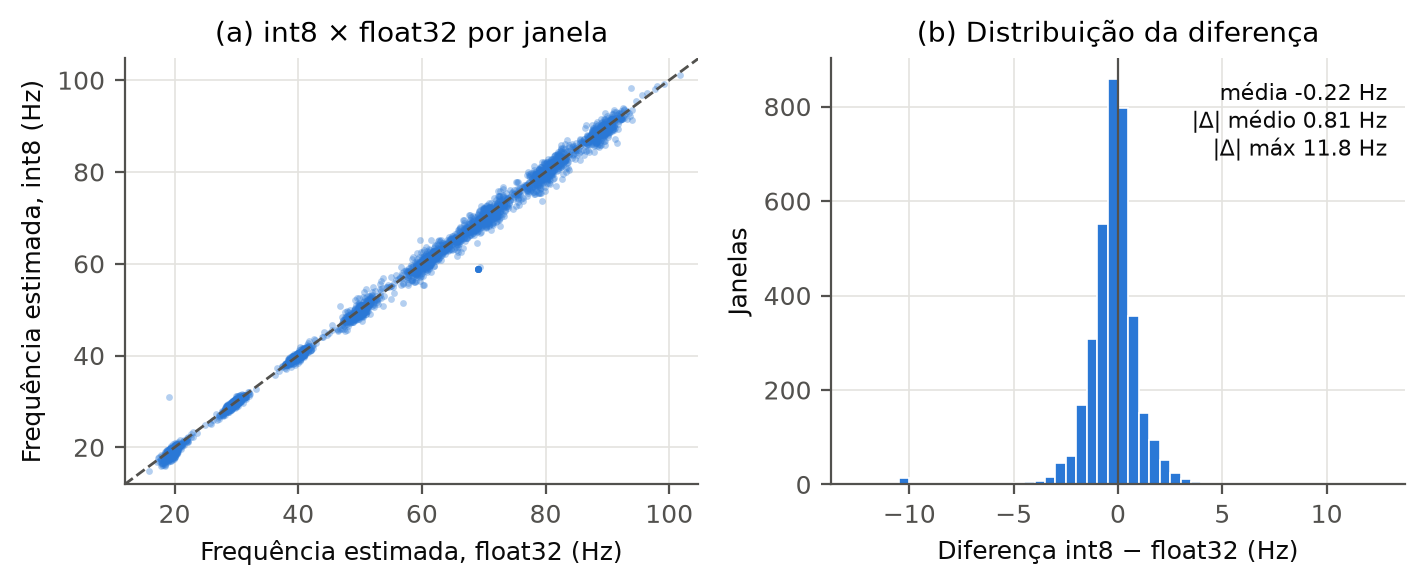
\includegraphics[width=\textwidth]{fig_quantizacao.png}
	\caption{Efeito da quantização int8 sobre a frequência estimada nas 3\,540 janelas: (a) estimativa int8 contra float32, com a reta identidade tracejada; (b) distribuição da diferença.}
	\label{fig:quantizacao}
\end{figure}

\begin{table}[htbp]
	\centering
	\small
	\caption{Concordância entre implementações (3\,540 janelas). ``Nível'' é a frequência arredondada a 10\,Hz.}
	\label{tab:fidelidade}
	\begin{tabular}{L{0.42\textwidth}ccc}
		\toprule
		\textbf{Comparação} & \textbf{Classe igual} & \textbf{Nível igual} & \textbf{\(|\Delta f|\) máx.} \\
		\midrule
		C float32 \(\times\) \texttt{scikit-learn} & 100\,\% & 100\,\% & \(2{,}5\times10^{-4}\)\,Hz \\
		C int8 \(\times\) emulação int8 (Python) & 100\,\% & 100\,\% & 0 (bit a bit) \\
		int8 \(\times\) float32 (efeito da quantização) & 98,2\,\% & 96,6\,\% & 11,8\,Hz \\
		Cadeia em C, percentis exatos \(\times\) Python int8 & 100\,\% & 100\,\% & 1,2\,Hz \\
		Cadeia em C, histograma \(\times\) Python int8 & 97,4\,\% & 96,2\,\% & 6,4\,Hz \\
		\bottomrule
	\end{tabular}
\end{table}

\subsection{Descritores e cadeia completa (V2)}

As fórmulas da Equação~\eqref{eq:conversao}, aplicadas aos campos brutos, reproduziram as colunas físicas do \texttt{hits.csv} com erro relativo de no máximo \(10^{-5}\), compatível com o arredondamento do próprio arquivo. A Figura~\ref{fig:descritores} mostra o erro normalizado máximo de cada descritor, nos dois canais, partindo do registro bruto. No modo exato, todos os erros ficaram abaixo de \(10^{-5}\), no nível da precisão simples; taxas e frações foram exatas, e os valores NaN coincidiram em todas as janelas. No modo histograma, os percentis ficaram acima da tolerância, como esperado de uma quantização em classes de largura fixa, com erros de até 0,2\,dB na amplitude, 0,04 nos logaritmos e 1,5\,kHz na frequência média.

\begin{figure}[htbp]
	\centering
	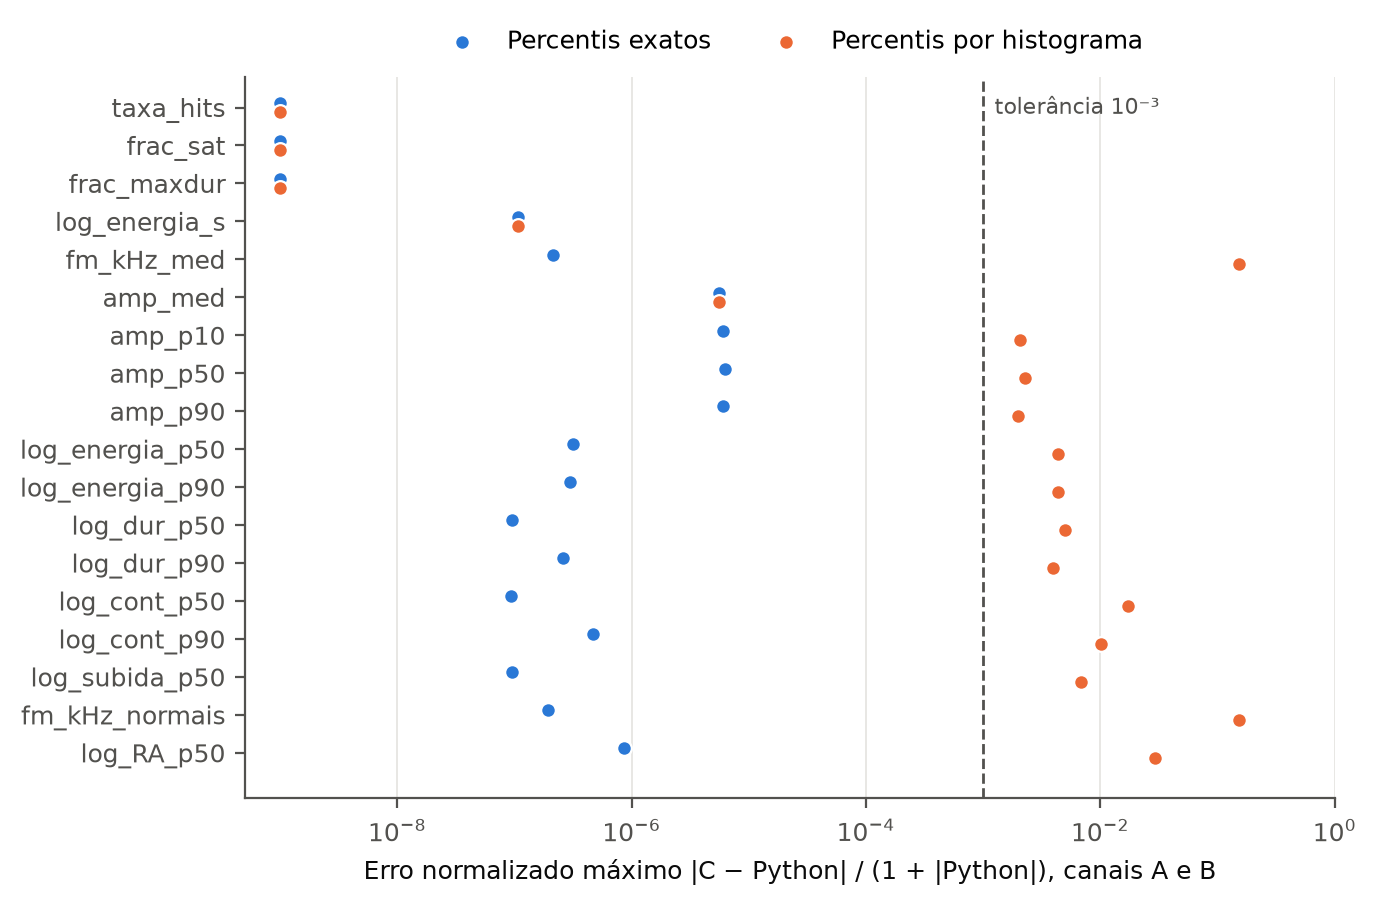
\includegraphics[width=0.92\textwidth]{fig_erro_descritores.png}
	\caption{Erro normalizado máximo, \(|x_{\mathrm{C}} - x_{\mathrm{Py}}|/(1+|x_{\mathrm{Py}}|)\), de cada descritor calculado em C a partir do registro bruto, nos dois modos de percentis, sobre as 3\,540 janelas e os dois canais. Erros nulos são desenhados em \(10^{-9}\). A linha tracejada é a tolerância de \(10^{-3}\).}
	\label{fig:descritores}
\end{figure}

O que importa para a aplicação é a saída das redes. Com percentis exatos, a cadeia completa em C devolveu a mesma classe e o mesmo nível de frequência que o Python em 100\,\% das janelas; a maior diferença de frequência, 1,2\,Hz, vem do arredondamento da amplitude no \texttt{hits.csv}, que o C não usa ao partir do registro bruto. Com histogramas, a classe coincidiu em 97,4\,\% e o nível em 96,2\,\% (Tabela~\ref{tab:fidelidade}), uma perda comparável à da própria quantização.

\subsection{Núcleo em lógica dedicada (V3 e V4)}

A simulação C e a cossimulação C/RTL do núcleo HLS, com 256 janelas, terminaram sem nenhuma divergência nos acumuladores ou na classe. A latência das duas redes foi de 11\,391 ciclos na síntese e de 11\,268 a 11\,393 ciclos na cossimulação, ou cerca de 114\,\(\mu\)s a 100\,MHz. Cada neurônio custa o número de entradas mais cerca de 12 ciclos de enchimento do \textit{pipeline}.

A Tabela~\ref{tab:recursos} compara a estimativa da síntese HLS com o resultado após posicionamento e roteamento fora de contexto. A temporização foi atendida com folga: o caminho crítico tem 6,84\,ns, o que admitiria cerca de 146\,MHz. A implementação ocupou bem menos LUTs que a estimativa (656 contra 2\,421), porque a síntese lógica absorve parte da lógica de controle, e mais DSPs (14 contra 10), por causa da multiplicação de 64 bits da requantização. Os 3,5 blocos de BRAM guardam os 8\,960 pesos int8 das duas redes.

\begin{table}[htbp]
	\centering
	\small
	\caption{Recursos do IP HLS no XC7A35T (100\,MHz).}
	\label{tab:recursos}
	\begin{tabular}{lrrrr}
		\toprule
		\textbf{Recurso} & \textbf{Estimativa HLS} & \textbf{Pós-roteamento} & \textbf{Disponível} & \textbf{Uso} \\
		\midrule
		LUT & 2\,421 & 656 & 20\,800 & 3,2\,\% \\
		\textit{Flip-flops} & 1\,648 & 682 & 41\,600 & 1,6\,\% \\
		DSP48E1 & 10 & 14 & 90 & 15,6\,\% \\
		BRAM (blocos de 36\,kb) & 3,5 & 3,5 & 50 & 7,0\,\% \\
		Período (ns) & 7,00 & 6,84 & 10,00 (alvo) & --- \\
		\bottomrule
	\end{tabular}
\end{table}

\subsection{Programa na MicroBlaze (V5)}

As seis simulações RTL (três programas \(\times\) duas configurações do processador) terminaram com a mesma sequência de valores de resultado da execução no computador: mesmas classes, mesmos acumuladores e, no modo exato, nenhum descritor fora da tolerância. Isso confirma, no nível do processador, que o binário embarcado reproduz o modelo. A Tabela~\ref{tab:ciclos} resume os ciclos medidos.

\begin{table}[htbp]
	\centering
	\small
	\caption{Ciclos medidos na simulação RTL da MicroBlaze (100\,MHz, memória local, sem caches). Com FPU, médias sobre 2 vetores (MLP) e 2 janelas reais com 163 \textit{hits} (cadeia); sem FPU, 1 vetor e 1 janela com 81 \textit{hits}.}
	\label{tab:ciclos}
	\begin{tabular}{lrr}
		\toprule
		\textbf{Etapa} & \textbf{Sem FPU} & \textbf{Com FPU} \\
		\midrule
		MLP float32, duas redes & \mbMlpFloatSoft & \mbMlpFloatFpu \\
		Quantização da entrada & \mbQuantSoft & \mbQuantFpu \\
		Núcleo int8, duas redes & \mbMlpIntSoft & \mbMlpIntFpu \\
		Inferência int8 completa (\(\mu\)s) & \mbMlpIntSoftUs & \mbMlpIntFpuUs \\
		\midrule
		Por \textit{hit}, modo exato & \mbHitSoft & \mbHitFpu \\
		Por \textit{hit}, modo histograma & \mbHitHistSoft & \mbHitHistFpu \\
		Fechar a janela, modo exato & \mbFecharSoft & \mbFecharFpu \\
		Fechar a janela, modo histograma & \mbFecharHistSoft & \mbFecharHistFpu \\
		\bottomrule
	\end{tabular}
\end{table}

\mbParagrafoMlp

A Figura~\ref{fig:latencia} compara a latência da inferência nas plataformas. A Figura~\ref{fig:ciclosjanela} decompõe o custo de uma janela típica dos dados (cerca de 80 \textit{hits}), e a Figura~\ref{fig:carga} extrapola, a partir dos ciclos medidos, a ocupação da CPU em função da taxa de \textit{hits}.

\begin{figure}[htbp]
	\centering
	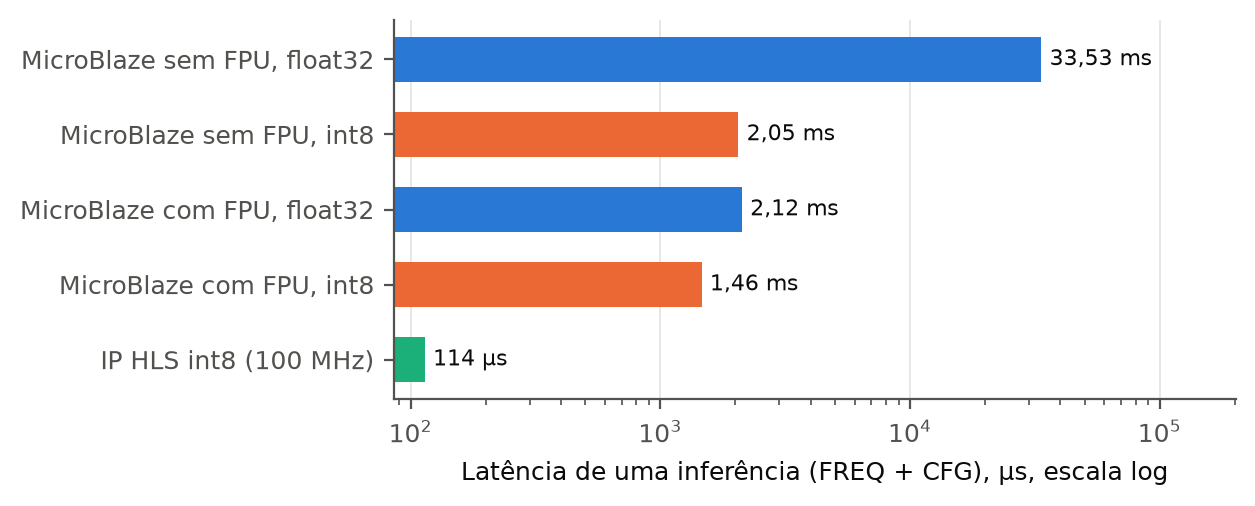
\includegraphics[width=0.85\textwidth]{fig_latencia_mlp.png}
	\caption{Latência de uma inferência (regressor e classificador) na MicroBlaze, medida em simulação RTL, e no IP HLS, medida na cossimulação. A MicroBlaze int8 inclui a quantização da entrada.}
	\label{fig:latencia}
\end{figure}

\begin{figure}[htbp]
	\centering
	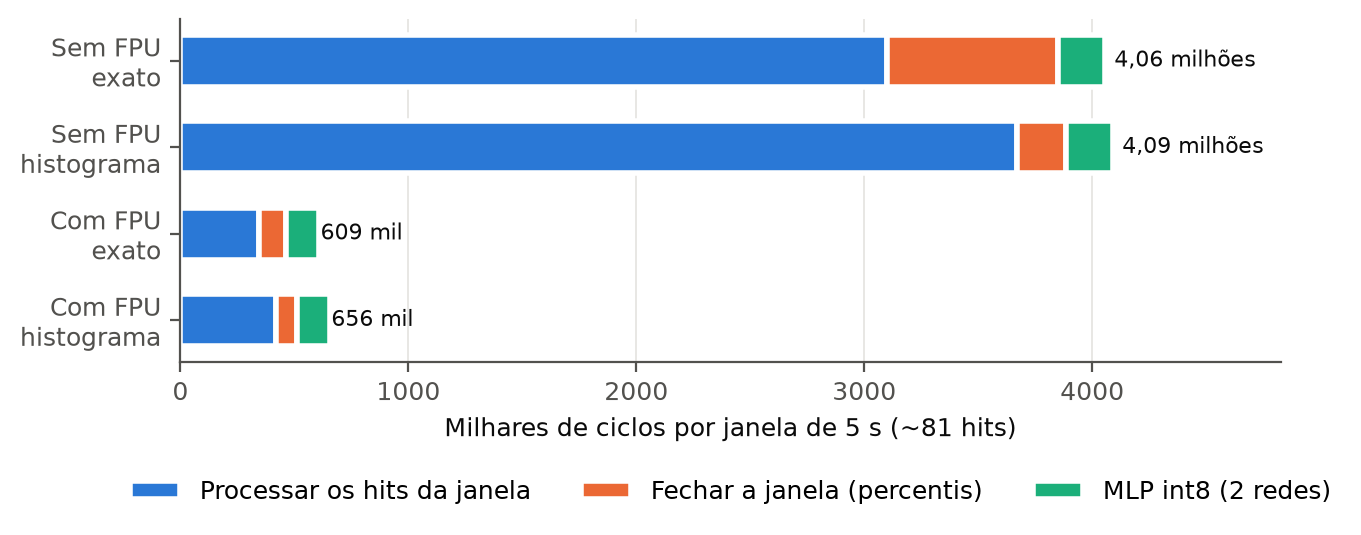
\includegraphics[width=0.92\textwidth]{fig_ciclos_janela.png}
	\caption{Composição dos ciclos de uma janela de 5\,s na MicroBlaze, para uma janela real de 81 \textit{hits} (custos por \textit{hit} medidos): processamento dos \textit{hits}, fechamento da janela (percentis) e MLP int8.}
	\label{fig:ciclosjanela}
\end{figure}

\begin{figure}[htbp]
	\centering
	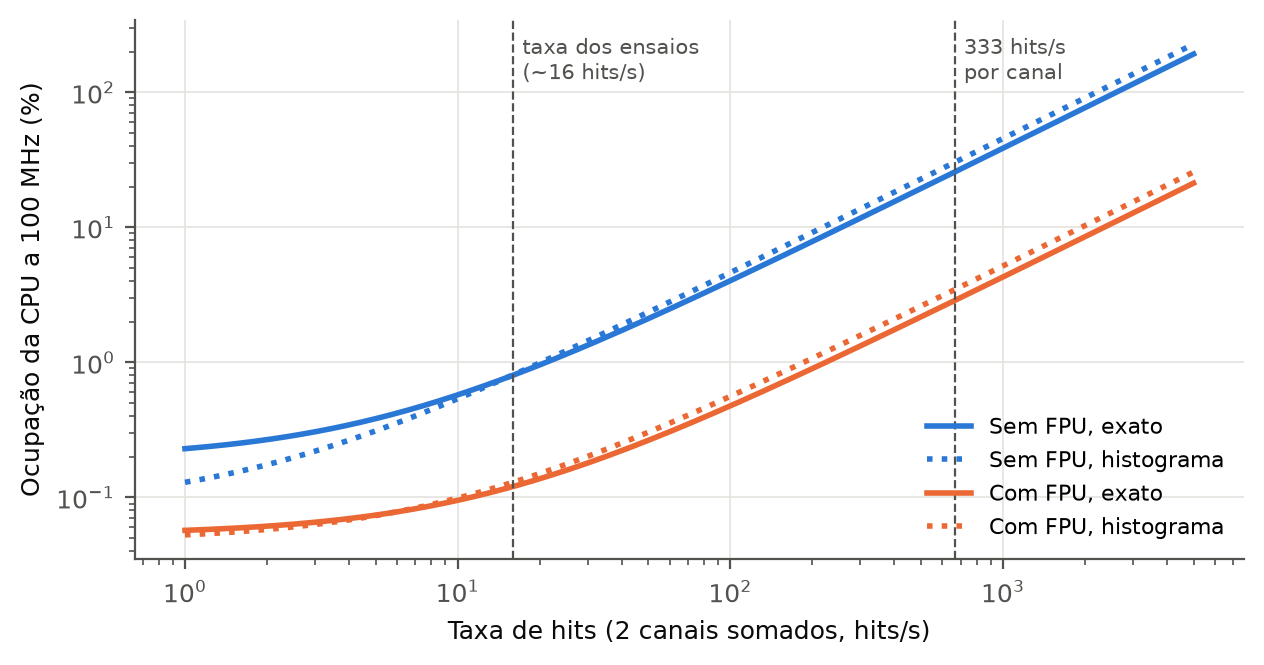
\includegraphics[width=0.85\textwidth]{fig_carga_cpu.png}
	\caption{Ocupação da CPU da MicroBlaze a 100\,MHz pela cadeia embarcada em função da taxa de \textit{hits}, extrapolada dos ciclos medidos por \textit{hit}, por fechamento de janela e pela MLP. As linhas verticais marcam a taxa dos ensaios da bomba e a maior taxa sustentada em ensaio elétrico. No modo exato, o fechamento da janela foi medido com cerca de 80 \textit{hits} e cresce como \(n \log n\); a extrapolação o subestima em taxas altas, e acima de 1\,024 \textit{hits} por canal por janela (cerca de 205 \textit{hits}/s por canal) o modo exato deixa de se aplicar.}
	\label{fig:carga}
\end{figure}

\mbParagrafoCarga

A Tabela~\ref{tab:memoria} resume a memória. O binário de teste da cadeia, com a MLP int8 e sem o caminho float32, ocupa de \mbTextoMin{} a \mbTextoMax\,kB de código e constantes, incluindo cerca de 10\,kB de \textit{hits} de teste que não existem no firmware real.

\begin{table}[htbp]
	\centering
	\small
	\caption{Memória da cadeia embarcada (ELF de teste, \texttt{mb-gcc} 2022.2, \texttt{-O2}).}
	\label{tab:memoria}
	\begin{tabular}{lrr}
		\toprule
		\textbf{Item} & \textbf{Sem FPU} & \textbf{Com FPU} \\
		\midrule
		Código e constantes, modo exato (kB) & \mbTextoExatoSoft & \mbTextoExatoFpu \\
		Código e constantes, modo histograma (kB) & \mbTextoHistSoft & \mbTextoHistFpu \\
		Estado da janela, modo exato (kB) & 65,6 & 65,6 \\
		Estado da janela, modo histograma (kB) & 10,3 & 10,3 \\
		Pesos int8 e vieses das duas redes (kB) & \(\approx 9{,}8\) & \(\approx 9{,}8\) \\
		Pesos float32 das duas redes, se usados (kB) & \(\approx 37\) & \(\approx 37\) \\
		\bottomrule
	\end{tabular}
\end{table}

% =======================================================================================================
\section{Discussão}
\label{sec:discussao}

\subsection{Qual rota usar}

A Tabela~\ref{tab:rotas} reúne o custo em lógica de cada alternativa. Os números da MicroBlaze vêm da síntese do mesmo sistema usado na simulação e servem para dimensionar o acréscimo da FPU; o processador em si já existe no MOMEA e não é um custo da cadeia.

\begin{table}[htbp]
	\centering
	\small
	\caption{Recursos lógicos no XC7A35T: núcleo da MicroBlaze (síntese) e IP HLS (pós-roteamento).}
	\label{tab:rotas}
	\begin{tabular}{lrrrr}
		\toprule
		\textbf{Bloco} & \textbf{LUT} & \textbf{FF} & \textbf{DSP} & \textbf{BRAM (36\,kb)} \\
		\midrule
		MicroBlaze sem FPU (núcleo) & 1\,361 & 857 & 4 & --- \\
		MicroBlaze com FPU estendida (núcleo) & 2\,322 & 1\,599 & 6 & --- \\
		Acréscimo da FPU & 961 & 742 & 2 & --- \\
		IP HLS int8 (duas redes) & 656 & 682 & 14 & 3,5 \\
		Memória local de 128\,kB (sistema simulado) & 17 & 16 & --- & 32 \\
		\bottomrule
	\end{tabular}
\end{table}

Para a aplicação atual, uma decisão a cada 5\,s, as duas rotas sobram. \mbParagrafoRota{} O IP HLS é \mbFatorHls{} vezes mais rápido que a MicroBlaze sem FPU e libera o processador, ao custo de 14 DSPs e 3,5 blocos de BRAM; ele se justificaria para classificar cada \textit{hit} em taxas altas, para modelos maiores ou se a MicroBlaze já estiver saturada pela pilha de rede. Em qualquer caso, a parte cara da cadeia não é a rede, mas o processamento por \textit{hit}, dominado pelos logaritmos; esse custo é o mesmo nas duas rotas, porque os descritores ficam no processador. Se a taxa de \textit{hits} crescer muito, o próximo passo natural é calcular na lógica as grandezas por \textit{hit} (incluindo os logaritmos, por tabela) e deixar à MicroBlaze apenas o fechamento da janela.

Entre os modos de percentis, o exato é preferível enquanto a janela couber na memória, porque preserva a decisão do modelo de referência em todas as janelas. O histograma troca cerca de 2,6\,\% de classes diferentes por memória constante e custo por \textit{hit} independente da taxa. Histogramas mais finos reduziriam essa diferença.

\subsection{O que a simulação garante}

A cadeia de verificação estabelece, com critérios explícitos, que: (i) a exportação do modelo e a implementação em C reproduzem o modelo de referência, bit a bit no caso int8; (ii) os descritores calculados em C a partir do registro bruto reproduzem os do estudo complementar; (iii) o RTL gerado pelo HLS é funcionalmente idêntico ao C e fecha a temporização na peça do MOMEA; e (iv) o binário compilado para a MicroBlaze produz os mesmos resultados em um processador simulado no nível RTL, com custo de tempo medido em ciclos.

A simulação não cobre, porém, o que depende da placa e do sistema completo:
\begin{itemize}
	\item a integração com o projeto atual do MOMEA, cuja ocupação de recursos não foi verificada; os recursos do IP foram obtidos fora de contexto, e o sistema MicroBlaze simulado não é o do MOMEA;
	\item o tempo de parede no firmware real, com caches ou memória externa, interrupções, recepção dos registros e pilha UDP concorrendo pelo processador;
	\item a base de tempo da janela: no treino, as janelas usaram a hora de chegada dos registros no computador; na placa, usarão o relógio local. Com o carimbo de tempo de \textit{hardware} ainda não implementado, pequenas diferenças na fronteira das janelas são esperadas;
	\item o comportamento elétrico do \textit{front-end} e do conversor, incluindo a saturação observada nos ensaios da bomba \cite{mlpbomba2026}.
\end{itemize}

\subsection{O modelo continua sendo o limite}

A implementação não muda a capacidade de generalização do modelo. No estudo complementar, a frequência generalizou para corridas não vistas (erro médio de 4 a 6\,Hz), mas a configuração das válvulas não (21 a 28\,\% de acurácia por corrida deixada de fora, para 14\,\% de acaso), e os dados têm limitações sérias: uma única corrida por condição, ordem fixa, limiar variável entre sessões e 70\,\% dos \textit{hits} saturados \cite{mlpbomba2026}. A contribuição deste trabalho é a infraestrutura: um fluxo que leva qualquer modelo do mesmo formato do Python ao FPGA, com verificação automática em cada nível. Retreinar com dados melhores exige apenas regenerar os cabeçalhos e repetir os testes; o código e o \textit{hardware} não mudam.

% =======================================================================================================
\section{Conclusões}
\label{sec:conclusoes}

A cadeia de classificação de condições de bomba por EA foi levada do computador para o FPGA do MOMEA e verificada inteiramente por simulação. O cálculo dos descritores em C, com percentis exatos, e as MLPs quantizadas para int8 reproduziram o modelo de referência em 100\,\% das 3\,540 janelas quanto à classe e ao nível de frequência; a quantização, isoladamente, alterou 1,8\,\% das classes e 0,81\,Hz da frequência em média. O núcleo int8, com fonte única, passou na cossimulação C/RTL e, como IP, ocupa cerca de 3\,\% das LUTs, 16\,\% dos DSPs e 7\,\% das BRAMs do XC7A35T, com 114\,\(\mu\)s por inferência. Na MicroBlaze simulada no nível RTL, o mesmo binário produziu resultados idênticos aos do computador, com a inferência int8 em \mbMlpIntSoftUs\,\(\mu\)s sem FPU e \mbMlpIntFpuUs\,\(\mu\)s com FPU, e a cadeia completa ocupa menos de \mbCargaEnsaioMax\,\% da CPU na taxa dos ensaios.

Os próximos passos, quando houver acesso às placas, são integrar a cadeia ao firmware do MOMEA, medir o tempo de parede com a pilha de rede ativa e validar o ciclo completo com sinais injetados e na bancada. Do lado do modelo, a prioridade é um novo ensaio com repetições, ordem aleatorizada, limiar fixo e ganho ajustado para evitar a saturação; os modelos resultantes entram no mesmo fluxo sem mudanças no código.

\section*{Reprodutibilidade}

Todo o fluxo está em \texttt{MLP/embarcado/}: \texttt{exportar\_modelo.py} e \texttt{exportar\_hits.py} geram os pesos, os vetores de teste e os \textit{hits}; \texttt{teste\_pc.bat} executa os níveis V1 e V2; \texttt{hls/run\_hls.tcl} e \texttt{hls/run\_hls\_impl.tcl} executam V3 e V4; e \texttt{microblaze/sim/rodar\_sim\_mb.py} compila os ELFs já gerados, monta o sistema MicroBlaze no Vivado e executa as simulações de V5. As figuras saem de \texttt{figuras\_sim.py}.

% =======================================================================================================
\begin{thebibliography}{99}

	\bibitem[AMD(2022a)]{amd_ug1399}
	AMD.
	\newblock \emph{Vitis High-Level Synthesis User Guide (UG1399)}, v2022.2.
	\newblock San Jose: Advanced Micro Devices, 2022.

	\bibitem[AMD(2022b)]{amd_ug984}
	AMD.
	\newblock \emph{MicroBlaze Processor Reference Guide (UG984)}, v2022.2.
	\newblock San Jose: Advanced Micro Devices, 2022.

	\bibitem[AMD(2022c)]{amd_ug900}
	AMD.
	\newblock \emph{Vivado Design Suite User Guide: Logic Simulation (UG900)}, v2022.2.
	\newblock San Jose: Advanced Micro Devices, 2022.

	\bibitem[Duarte et al.(2018)]{duarte2018}
	DUARTE, J. et al.
	\newblock Fast inference of deep neural networks in FPGAs for particle physics.
	\newblock \emph{Journal of Instrumentation}, v. 13, n. 7, P07027, 2018.
	\newblock DOI: \href{https://doi.org/10.1088/1748-0221/13/07/P07027}{10.1088/1748-0221/13/07/P07027}.

	\bibitem[Goldberg(1991)]{goldberg1991}
	GOLDBERG, D.
	\newblock What every computer scientist should know about floating-point arithmetic.
	\newblock \emph{ACM Computing Surveys}, v. 23, n. 1, p. 5--48, 1991.
	\newblock DOI: \href{https://doi.org/10.1145/103162.103163}{10.1145/103162.103163}.

	\bibitem[Hyndman e Fan(1996)]{hyndman1996}
	HYNDMAN, R. J.; FAN, Y.
	\newblock Sample quantiles in statistical packages.
	\newblock \emph{The American Statistician}, v. 50, n. 4, p. 361--365, 1996.
	\newblock DOI: \href{https://doi.org/10.1080/00031305.1996.10473566}{10.1080/00031305.1996.10473566}.

	\bibitem[IEEE(2019)]{ieee754}
	IEEE.
	\newblock \emph{IEEE Standard for Floating-Point Arithmetic} (IEEE Std 754-2019).
	\newblock New York: IEEE, 2019.

	\bibitem[Jacob et al.(2018)]{jacob2018}
	JACOB, B.; KLIGYS, S.; CHEN, B.; ZHU, M.; TANG, M.; HOWARD, A.; ADAM, H.; KALENICHENKO, D.
	\newblock Quantization and training of neural networks for efficient integer-arithmetic-only inference.
	\newblock In: \emph{IEEE/CVF Conference on Computer Vision and Pattern Recognition (CVPR)}, 2018. p. 2704--2713.

	\bibitem[Krishnamoorthi(2018)]{krishnamoorthi2018}
	KRISHNAMOORTHI, R.
	\newblock Quantizing deep convolutional networks for efficient inference: a whitepaper.
	\newblock arXiv:1806.08342, 2018.

	\bibitem[Autores(2026)]{mlpbomba2026}
	AUTORES.
	\newblock Classificação das condições de operação de uma bomba por emissão acústica: redes MLP, florestas aleatórias e \textit{gradient boosting} sobre \textit{hits} extraídos em FPGA, com validação por corrida.
	\newblock Relatório técnico, 2026.

	\bibitem[Nagel et al.(2021)]{nagel2021}
	NAGEL, M.; FOURNARAKIS, M.; AMJAD, R. A.; BONDARENKO, Y.; VAN BAALEN, M.; BLANKEVOORT, T.
	\newblock A white paper on neural network quantization.
	\newblock arXiv:2106.08295, 2021.

	\bibitem[Ohno e Ohtsu(2010)]{ohno2010}
	OHNO, K.; OHTSU, M.
	\newblock Crack classification in concrete based on acoustic emission.
	\newblock \emph{Construction and Building Materials}, v. 24, n. 12, p. 2339--2346, 2010.
	\newblock DOI: \href{https://doi.org/10.1016/j.conbuildmat.2010.05.004}{10.1016/j.conbuildmat.2010.05.004}.

	\bibitem[Pedregosa et al.(2011)]{pedregosa2011}
	PEDREGOSA, F. et al.
	\newblock Scikit-learn: machine learning in Python.
	\newblock \emph{Journal of Machine Learning Research}, v. 12, p. 2825--2830, 2011.

	\bibitem[Prechelt(1998)]{prechelt1998}
	PRECHELT, L.
	\newblock Early stopping -- but when?
	\newblock In: ORR, G. B.; MÜLLER, K.-R. (ed.). \emph{Neural Networks: Tricks of the Trade}.
	\newblock Berlin: Springer, 1998. (Lecture Notes in Computer Science, v. 1524). p. 55--69.

	\bibitem[Unn{\th}{\'o}rsson(2013)]{unnthorsson2013}
	UNN{\TH}{\'O}RSSON, R.
	\newblock Hit detection and determination in AE bursts.
	\newblock In: SIKORSKI, W. (ed.). \emph{Acoustic Emission---Research and Applications}.
	\newblock Rijeka: IntechOpen, 2013.
	\newblock DOI: \href{https://doi.org/10.5772/54754}{10.5772/54754}.

	\bibitem[Vallen Systeme(2022)]{vallen2022}
	VALLEN SYSTEME GMBH.
	\newblock \emph{AMSY-6: System Specification}.
	\newblock Wolfratshausen: Vallen Systeme GmbH, 2022.

\end{thebibliography}

\end{document}
